%%
%% Copyright 2007, 2008, 2009 Elsevier Ltd
%%
%% This file is part of the 'Elsarticle Bundle'.
%% ---------------------------------------------
%%
%% It may be distributed under the conditions of the LaTeX Project Public
%% License, either version 1.2 of this license or (at your option) any
%% later version.  The latest version of this license is in
%%    http://www.latex-project.org/lppl.txt
%% and version 1.2 or later is part of all distributions of LaTeX
%% version 1999/12/01 or later.
%%
%% The list of all files belonging to the 'Elsarticle Bundle' is
%% given in the file `manifest.txt'.
%%

%% Template article for Elsevier's document class `elsarticle'
%% with numbered style bibliographic references
%% SP 2008/03/01
%%
%%
%%
%% $Id: elsarticle-template-num.tex 4 2009-10-24 08:22:58Z rishi $
%%
%%
\documentclass[preprint,12pt]{elsarticle}

%% Use the option review to obtain double line spacing
%% \documentclass[preprint,review,12pt]{elsarticle}

%% Use the options 1p,twocolumn; 3p; 3p,twocolumn; 5p; or 5p,twocolumn
%% for a journal layout:
%% \documentclass[final,1p,times]{elsarticle}
%% \documentclass[final,1p,times,twocolumn]{elsarticle}
%% \documentclass[final,3p,times]{elsarticle}
%% \documentclass[final,3p,times,twocolumn]{elsarticle}
%% \documentclass[final,5p,times]{elsarticle}
%% \documentclass[final,5p,times,twocolumn]{elsarticle}

%% if you use PostScript figures in your article
%% use the graphics package for simple commands
%% \usepackage{graphics}
%% or use the graphicx package for more complicated commands
%% \usepackage{graphicx}
%% or use the epsfig package if you prefer to use the old commands
%% \usepackage{epsfig}

%% The amssymb package provides various useful mathematical symbols
\usepackage{amssymb}
%% The amsthm package provides extended theorem environments
%% \usepackage{amsthm}

%% The lineno packages adds line numbers. Start line numbering with
%% \begin{linenumbers}, end it with \end{linenumbers}. Or switch it on
%% for the whole article with \linenumbers after \end{frontmatter}.
%% \usepackage{lineno}

%% natbib.sty is loaded by default. However, natbib options can be
%% provided with \biboptions{...} command. Following options are
%% valid:

%%   round  -  round parentheses are used (default)
%%   square -  square brackets are used   [option]
%%   curly  -  curly braces are used      {option}
%%   angle  -  angle brackets are used    <option>
%%   semicolon  -  multiple citations separated by semi-colon
%%   colon  - same as semicolon, an earlier confusion
%%   comma  -  separated by comma
%%   numbers-  selects numerical citations
%%   super  -  numerical citations as superscripts
%%   sort   -  sorts multiple citations according to order in ref. list
%%   sort&compress   -  like sort, but also compresses numerical citations
%%   compress - compresses without sorting
%%
%% \biboptions{comma,round}

% \biboptions{}


\journal{Intelligent Data Analysis (extended)}

\begin{document}

\begin{frontmatter}

%% Title, authors and addresses

%% use the tnoteref command within \title for footnotes;
%% use the tnotetext command for the associated footnote;
%% use the fnref command within \author or \address for footnotes;
%% use the fntext command for the associated footnote;
%% use the corref command within \author for corresponding author footnotes;
%% use the cortext command for the associated footnote;
%% use the ead command for the email address,
%% and the form \ead[url] for the home page:
%%
%% \title{Title\tnoteref{label1}}
%% \tnotetext[label1]{}
%% \author{Name\corref{cor1}\fnref{label2}}
%% \ead{email address}
%% \ead[url]{home page}
%% \fntext[label2]{}
%% \cortext[cor1]{}
%% \address{Address\fnref{label3}}
%% \fntext[label3]{}

\title{Template for Intelligent Data Analysis (extended) assignment report}

%% use optional labels to link authors explicitly to addresses:
%% \author[label1,label2]{<author name>}
%% \address[label1]{<address>}
%% \address[label2]{<address>}

\author{A Student (Student ID: 123456)}

\address{School of Computer Science, University of Birmingham}

\begin{abstract}
Text of abstract

\end{abstract}

\begin{keyword}
%% keywords here, in the form: keyword \sep keyword

%% MSC codes here, in the form: \MSC code \sep code
%% or \MSC[2008] code \sep code (2000 is the default)

\end{keyword}

\end{frontmatter}

%%
%% Start line numbering here if you want
%%
% \linenumbers

%% main text
\section{Introduction}
\label{s:introduction}
This is the introduction.  Here is a reference to \cite{baber2017}.
\section{Assignment}
\label{s:assignment}
%
\subsection{Submission deadline}
\label{ss:deadline}
The submission deadline for this assignment is 5pm on Friday 8th March (week 8).
%
\subsection{Assignment details}
\label{ss:details}
You can chose any of the data set(s) from the list bellow, but finding your own dataset to investigate is much preferable!  For example, there are many potential text data sets (Twitter, online reviews, etc) and these can be converted to vector format using methods from the course.

If you decide to go the easier route and use some of the data sets provided, un-tar the relevant file and go to the corresponding folder.  The folder contains the data set, as well as additional information about the data. Read the available information, especially the description of the features (data dimensions).

Depending on the software that you use you will need to clean the data, for example so that it contains only numerical features (dimensions) and the features are space-separated (not comma-separated).

To make the plots informative, you should come up with a labeling scheme for data points.
If the data can be classified into several classes (find out in the data and feature description!), use that information as the basis for your labeling scheme. In that case exclude the class information from the data dimensions that you analyse.  Alternatively, you can make labels out of any dimension, e.g. by quantising it into several intervals. For example, if the data dimension represents age of a person, you can quantise it into 5 labels (classes) [child, teenager, young adult, middle age, old].  Associate the data labels with different markers and use the markers to show what kind of data points get projected to different regions of the visualization plot.

Learn as much as you can about an assigned data set(s) using the visualization and clustering methods developed in the module.
Use various data labeling schemes.
In the case of visualization, compare PCA with straightforward co-ordinate projections
Data sets:

\begin{itemize}
    \item abalone
    \item boston
    \item comp.activ
    \item image
    \item iris
    \item letter
\end{itemize}

Before starting to work on the assignment, please carefully study the example that Dr Tino prepared using the boston database. Un-tar the file boston.ex.tar.gz and go to the folder ``BOSTON.EX''.   The sub-folder ``FIGURES'' contains all the relevant figures as eps or gif files. Please consult the ``boston.read.me'' file in BOSTON.EX.

The report should describe experiments with a chosen data set(s) along the lines of the ``boston'' example.  In the labeling scheme, concentrate on more than one coordinate (dimension), e.g. in the ``boston'' example don't just consider the `price' feature, but run separate experiments with `per capita crime rate in the town', or 'pupil-teacher ratio in the town' instead of the `price' coordinate.
\subsection{Marking scheme}
\label{ss:marking}
In the report concentrate on the following questions:
\begin{itemize}
    \item How did you pre-process the data? (worth 20%)
    \item What features (coordinates) did you use for labeling the projected points with different markers? (worth 10%)
    \item How did you design the labeling schemes? (worth 20%)
    \item What interesting aspects of the data did you detect based on the data visualisations? (worth 30%)
    \item What interesting aspects of the data did you detect based on eigenvector and eigenvalue analysis of the data covariance matrix? (worth 20%)
\end{itemize}
You should demonstrate that you
\begin{itemize}
    \item Understand the visualisation techniques used
    \item Are able to extract useful information about otherwise inconceivable high-dimensional data using dimensionality-reducing visualisation techniques.
    \item The overall mark m (in the range 0-100\%) will be linearly scaled to the range 0-20\% by 0.2*m.
\end{itemize}
For examples of nice past reports developed on the "wine dataset" (do not use this data in your report!), please see reports by Christoph Stich and Josephf Preece.

\section{Acknowledgement}
\label{s:acknowledge}
I would like to thank Dr Peter Tino for permission to use this assignment, and Christoph Stich and Joseph Preece for their example reports.

\section{Including figures}
\label{s:another-section}
Here is a figure:
\begin{figure}[ht]
    \centerline{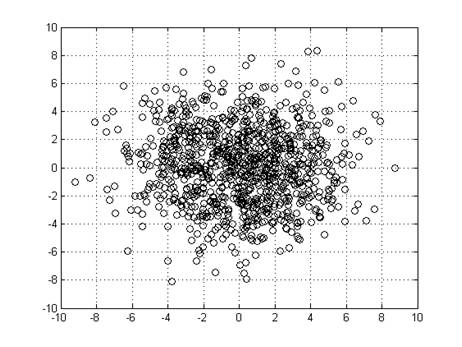
\includegraphics[scale=0.8]{figs/clus1.jpg}}
    \caption{An example figure (JPG)}
\end{figure}

%% The Appendices part is started with the command \appendix;
%% appendix sections are then done as normal sections
%% \appendix

%% \section{}
%% \label{}

%% References
%%
%% Following citation commands can be used in the body text:
%% Usage of \cite is as follows:
%%   \cite{key}         ==>>  [#]
%%   \cite[chap. 2]{key} ==>> [#, chap. 2]
%%

%% References with bibTeX database:

\bibliographystyle{elsarticle-num}
%\bibliography{<your-bib-database>}

%% Authors are advised to submit their bibtex database files. They are
%% requested to list a bibtex style file in the manuscript if they do
%% not want to use elsarticle-num.bst.

%% References without bibTeX database:

\begin{thebibliography}{00}

%% \bibitem must have the following form:
%%   \bibitem{key}...
%%

\bibitem{baber2017} Baber, C., Russell, M., Wing, A., Hermsdorfer, J. \& Khattab, A, {\em Creating Affording Situations: Coaching through Animate Objects}, Sensors, {\bf 17}, 2308, 2017

\end{thebibliography}


\end{document}

%%
%% End of file `elsarticle-template-num.tex'.
